% 01_feedback_schema.png

\chapter{Introduction}

The core model by which we understand economic processes is the interaction of and supply and
demand. This model has been considerably succesful in understanding why markets tend towards
equilibrium equality of supply and demand, but has failed to explain the remarkable persistence of
an excess of aggregate supply as indicated by a sustained and positive rate of unemployment.

In 1777 David Hume observed, despite theoretical considerations to the contrary, that properties of
a nation's currency had observable affects on the state of the economy,

\begin{quotation}
If we consider any one kingdom by itself, it is evident, that the greater or less plenty of money is
    of no consequence; since the prices of commodities are always proportioned to the plenty of
    money, and a crown in Harry VII.’s time served the same purpose as a pound does at present ...
    It is indeed evident, that money is nothing but the representation of labour and commodities,
    and serves only as a method of rating or estimating them. Where coin is in greater plenty; as a
    greater quantity of it is required to represent the same quantity of goods; it can have no
    effect, either good or bad, taking a nation within itself; any more than it would make an
    alteration on a merchant’s books, if, instead of the Arabian method of notation, which requires
    few characters, he should make use of the Roman, which requires a great many ... \textbf{But notwithstanding this conclusion}, which must be allowed just, it is certain, that, since the
    discovery of the mines in America, industry has encreased in all the nations of Europe, except
    in the possessors of those mines; and this may justly be ascribed, amongst other reasons, to the
    encrease of gold and silver.  Accordingly we find, that, in every kingdom, into which money
    begins to flow in greater abundance than formerly, every thing takes a new face: labour and
    industry gain life; the merchant becomes more enterprising, the manufacturer more diligent and
    skilful, and even the farmer follows his plough with greater alacrity and attention. This is not
    easily to be accounted for, if we consider only the influence which a greater abundance of coin
    has in the kingdom itself, by heightening the price of commodities, and obliging every one to
    pay a greater number of these little yellow or white pieces for every thing he purchases.
\end{quotation}

A simple model that aggregates equilibria in each market implies an equilibrium at the macro-level.
This model suggests macro-economic conditions as shown in Figure
\ref{fig:supply_and_demand_prediction}.

\begin{figure}
\centering

\includegraphics{example}
\caption{Supply and Demand Model Prediction}
\label{fig:supply_and_demand_prediction}
\end{figure}

However, contrary to Figure \ref{fig:supply_and_demand_prediction} which implies full-employment
Figure \ref{fig:ui_all_data} shows a vastly differing results.

\begin{figure}
\centering

\includegraphics{example}
\caption{Inflation Rate vs. Unemployment Data}
\label{fig:ui_all_data}
\end{figure}

\begin{figure}
\centering

\includegraphics{example}
\caption{Unemployment vs. Inflation Rate}
\label{fig:ui}
\end{figure}

Considering that any currency mechanism is absent from this model of supply and demand is seems
reasonable to find a way to include currency in our model. This leads to the question of what
methods should be used to analyze the properties of currency.

The fundamental insight that we present is that because currency is a digital system, the way to
approach its analysis is roughly analogous to the way we approach the analysis and design of other
digital systems (the internet being an interesting case in point), i.e. that we should approach the
analysis of currency as an engineering problem, and in particular the engineering and control of
dynamic systems. 

Economic theory approaches economic problems similarly to the way medicine treats the human body, by
applying relatively small changes, such as medicine, in response to various pathologies.
Destructuring and rebuilding biological systems is impossible. Importantly however, the control
system for economies, the currency, can indeed be destructured and rebuilt from first principles.
Thus we take a different approach, viewing the economic problem more like a robotics problem,
something that can be built from the bottom up, completely to our own specification, viewing
currency as an engineering control systems problem. To introduce the notion of a control system,
Figure \ref{fig:feedback_schema} shows the standard schema for a univariate single input single
output (SISO) control system. This approach is now possible due to the advances in digital
technologies and the relative ease in which a new digital currency can be designed, built and
tested, compared to the practical and technical limitations in applying similar solutions to paper
currencies.

The key components in the analysis and design of a digital currency are:

a) Understand the system as much as possible by break the system down into the correct components
and understanding as much as possible the interactions between the components.

b) Understand as much as possible the Control the components by isolating them and regulating their
interactions.

b) Understand as much as possible the  negative feedback processes that could be utilizied to
stabilize the system and reach desired state,

c) Understand as much as possible the positive feedback processes that may cause instability and
break the system,

d) Understand as much as possible how to compensate for the thermodynamic deterioration in the
system, or componensate for errors,

e) Understand as much as possible ways to prevent internal or external interactions from causing instability.

\subsection{Destructuring and Negative Feedback}

\begin{figure}
\includegraphics[scale=0.28]{/01/feedback_schema}
\caption{Control System Schema}
\label{fig:feedback_schema}
\end{figure}

A simple example of a control system is a thermostat which adjusts the heating of a room. Some
condition of the plant (the thing we want to control) is controlled by measuring the state of the
plant and feeding back into the plant the difference between this state and the desired state (the
reference signal). The design of control systems have the general guiding properties that dictate
our design approach, namely that our ability to correctly model the plant, stems must be able to
correct for errors, noise and/or energy disipation in the plant and the the minimum number of
control variables is determined by the number of variables that the control system seeks to control.
A control system for the economy looks like Figure \ref{fig:economic_feedback_schema}.

\begin{figure}
\centering
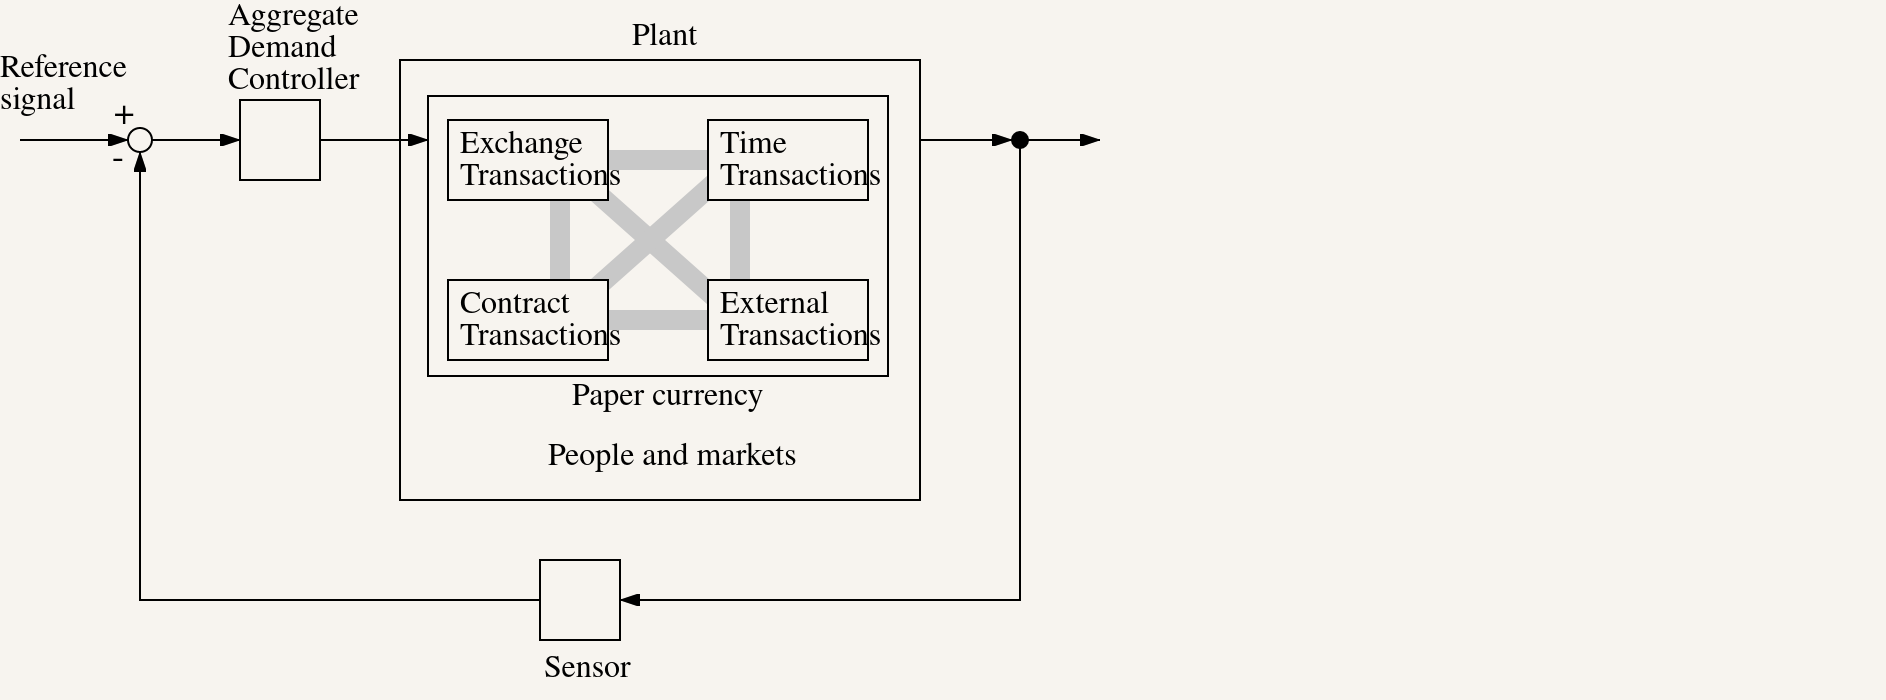
\includegraphics[scale=0.28]{/01/economic_feedback_schema}
\caption{Control System Schema for an Economy}
\label{fig:economic_feedback_schema}
\end{figure}

Zooming into the currency box in Figure \ref{fig:economic_feedback_schema}, we can specify the
classes of transactions that a currency implements. Transaction classes include the exchange of
money in return for goods or services, lending money now in exchange for payment later, and
exchanging money in exchange for a change in a contract. This way of viewing currency indicates a
control problem because the system has a single means to control money supply, but at least four
classes of components that require control and interact with the other classes.

\subsubsection{Control Problem}

\begin{figure}
\centering

\includegraphics{example}
\caption{Control Problem}
\label{fig:control_problem}
\end{figure}

The passing around of paper currency, in conjunction with contract agreements, is used to carry
out many kinds of transactions, the four main classes we term exchange transactions, time
transactions, contract transactions and external transacation. Each class of transaction interacts
with the other classes in complex ways. The fundamental problem is that these interactions are
overly complex to control with a single control such as control of the money supply. In general,
control systems require one control variable for each property of the plant that requires control.
This is implicit in the name of control systems, SISO for single input single output, MIMO for
multiple input multiple output. We therefore take a systematic approach to this control problem,
destructuring each transaction class and examining the way it interacts with other transactions
classes, step by step.

\begin{figure}
\centering
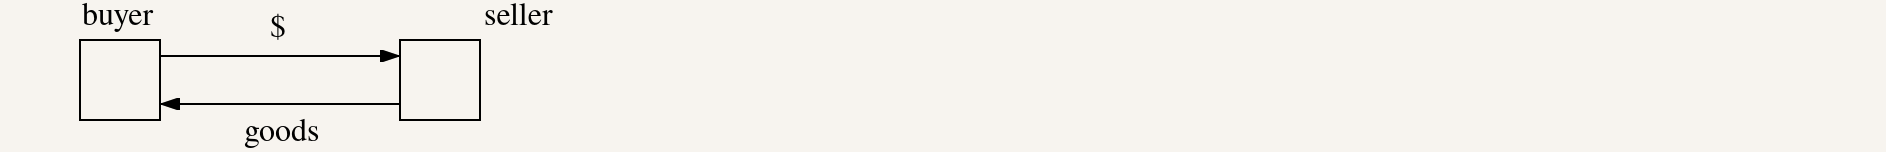
\includegraphics[scale=0.28]{/01/exchange_transactions}
\caption{Exchange Transactions}
\label{fig:exchange_transactions}
\end{figure}

\begin{figure}
\centering

\includegraphics{example}
\caption{Time Transactions}
\label{fig:time_transactions}
\end{figure}

\begin{figure}
\centering
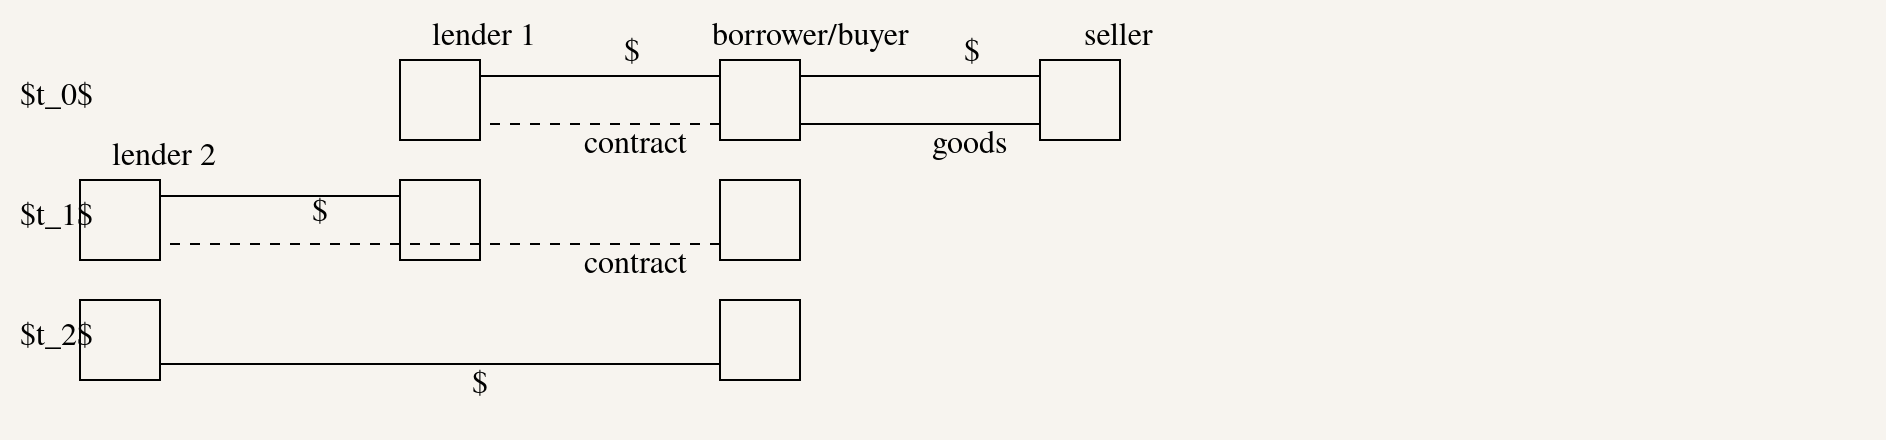
\includegraphics[scale=0.28]{/01/contract_transactions}
\caption{Contract Transactions}
\label{fig:contract_transactions}
\end{figure}

\begin{figure}
\centering
\includegraphics[scale=0.28]{/01/external_transactions}
\caption{External Transactions}
\label{fig:external_transactions}
\end{figure}

\section{Error Correction}

\begin{figure}
\centering
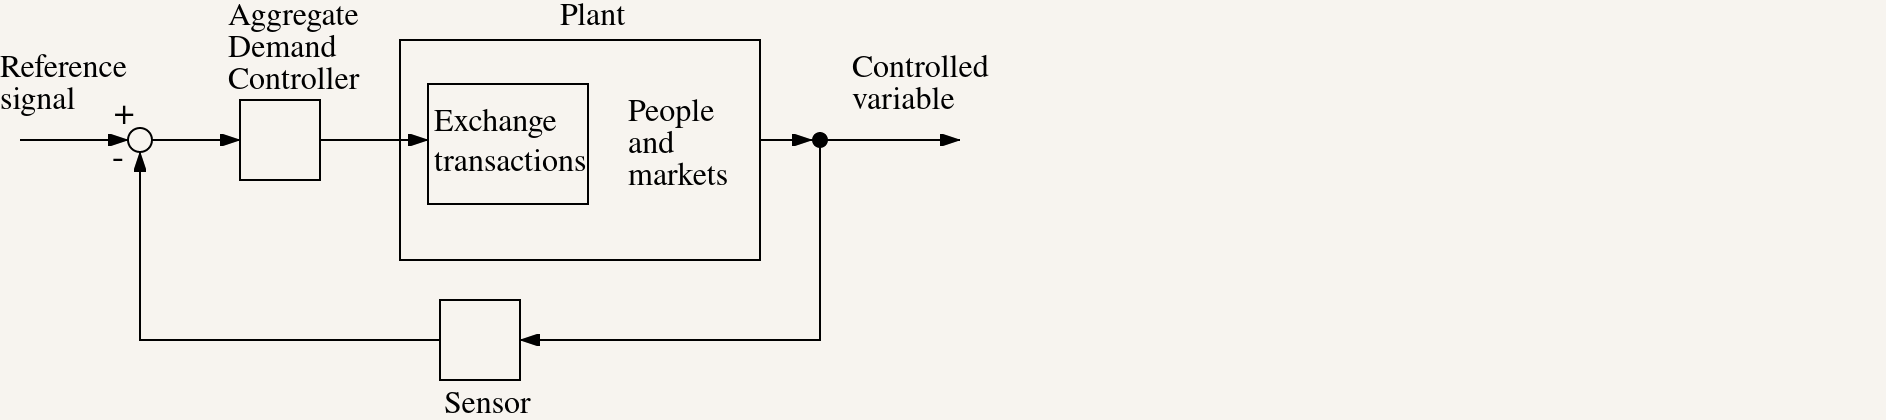
\includegraphics[scale=0.28]{/01/exchange_only_feedback_schema}
\caption{Exchange Only Feedback Model}
\label{fig:exchange_only_feedback_schema}
\end{figure}

Considering an economy where all other transaction categories have been eliminated, as
indicated in figure 1.11, we can build a simple aggregate model as shown in figure 1.12.

\begin{figure}
\centering
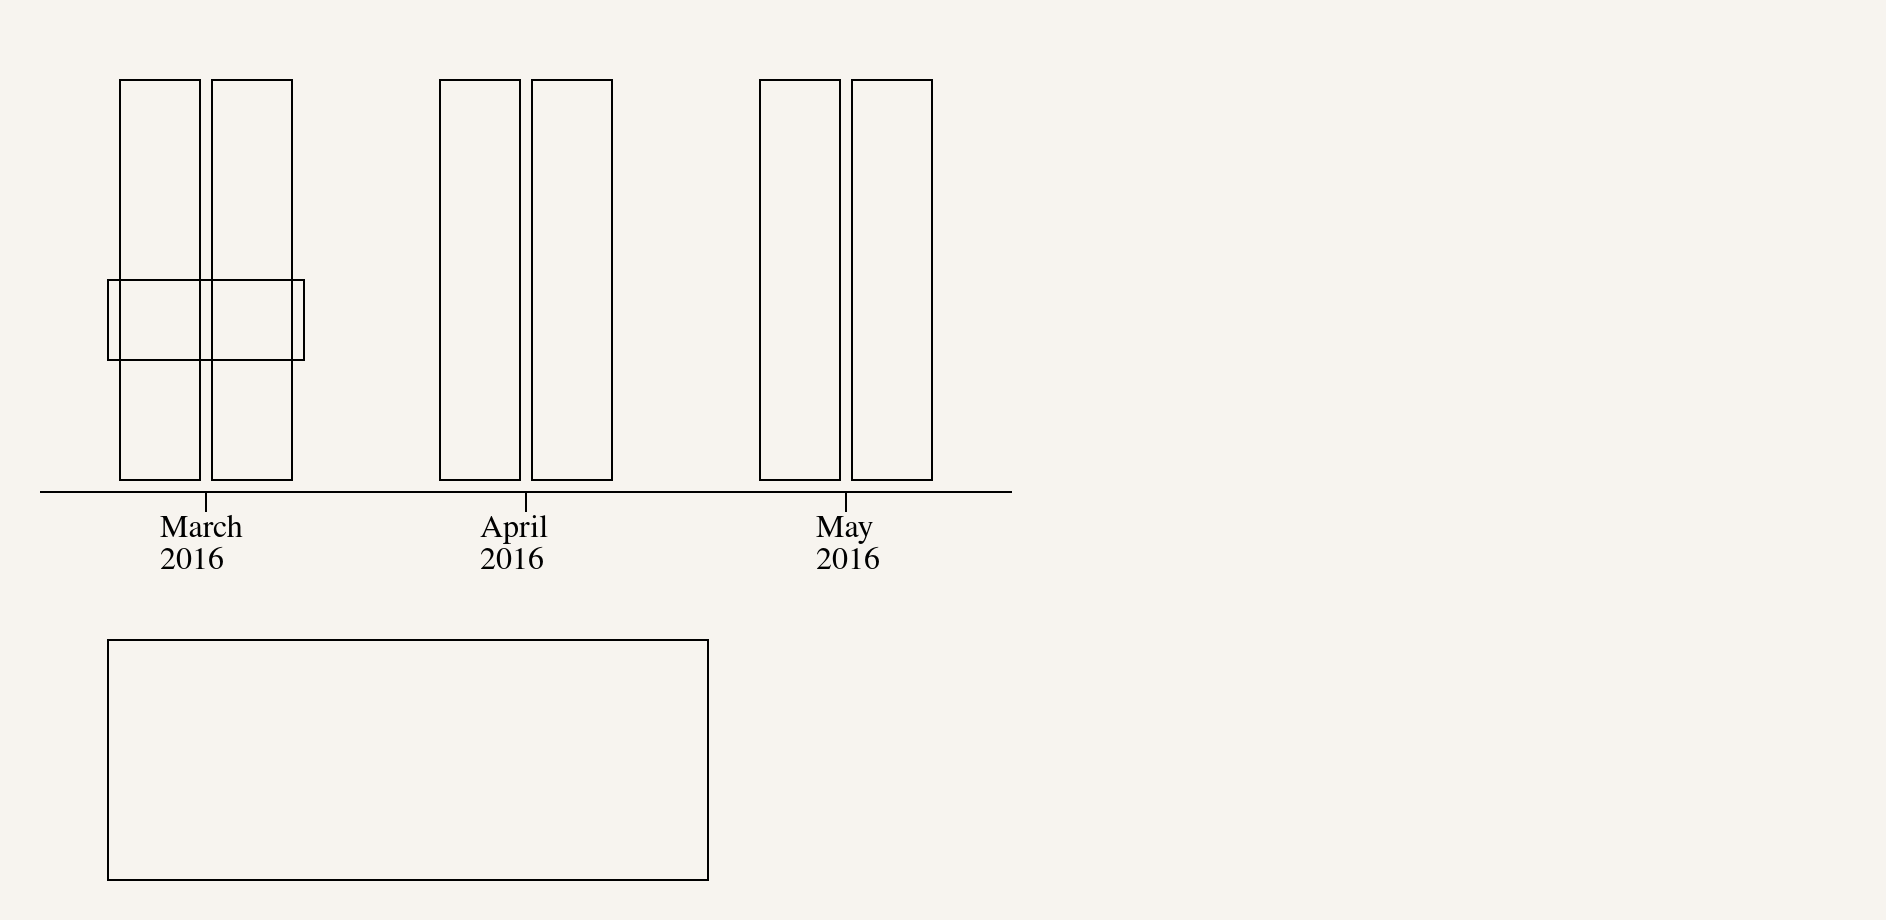
\includegraphics[scale=0.28]{/01/exchange_only_aggregate_model}
\caption{Exchange Only Aggregate Model}
\label{fig:exchange_only_aggregate_model}
\end{figure}

In periods 1 and 3, the unemployment rate, disregarding frictional unemployment, is zero.

So far the model is not constrained in any way. We apply to it an approximation of market behaviour,
assuming that, in the absence of the monetary authority changing money supply and hence aggregate
deman, that in each time period, the aggregate of prices \(p_i\) and quantities \(q_i\) adjust to
market equilibrium, i.e. that there is not excess aggregate suppl7y or excess aggregate demand. We
now have a model which is the same as the 'simple model' we presented earlier.

\begin{figure}
\centering

\includegraphics{example}
\caption{Equilibrium Aggregate Model}
\label{fig:equilibrium_aggregate_model}
\end{figure}

\begin{figure}
\centering

\includegraphics[scale=0.28]{/01/information_transmission}
\caption{Information Transmission and Coding}
\label{fig:information_transmission}
\end{figure}

\begin{figure}
\centering

\includegraphics{example}
\caption{Overbooking Model}
\label{fig:overbooking}
\end{figure}

\begin{figure}
\centering

\includegraphics{example}
\caption{Aggregate Model with Overbooking}
\label{fig:aggregate_overbooking}
\end{figure}

\begin{figure}
\centering
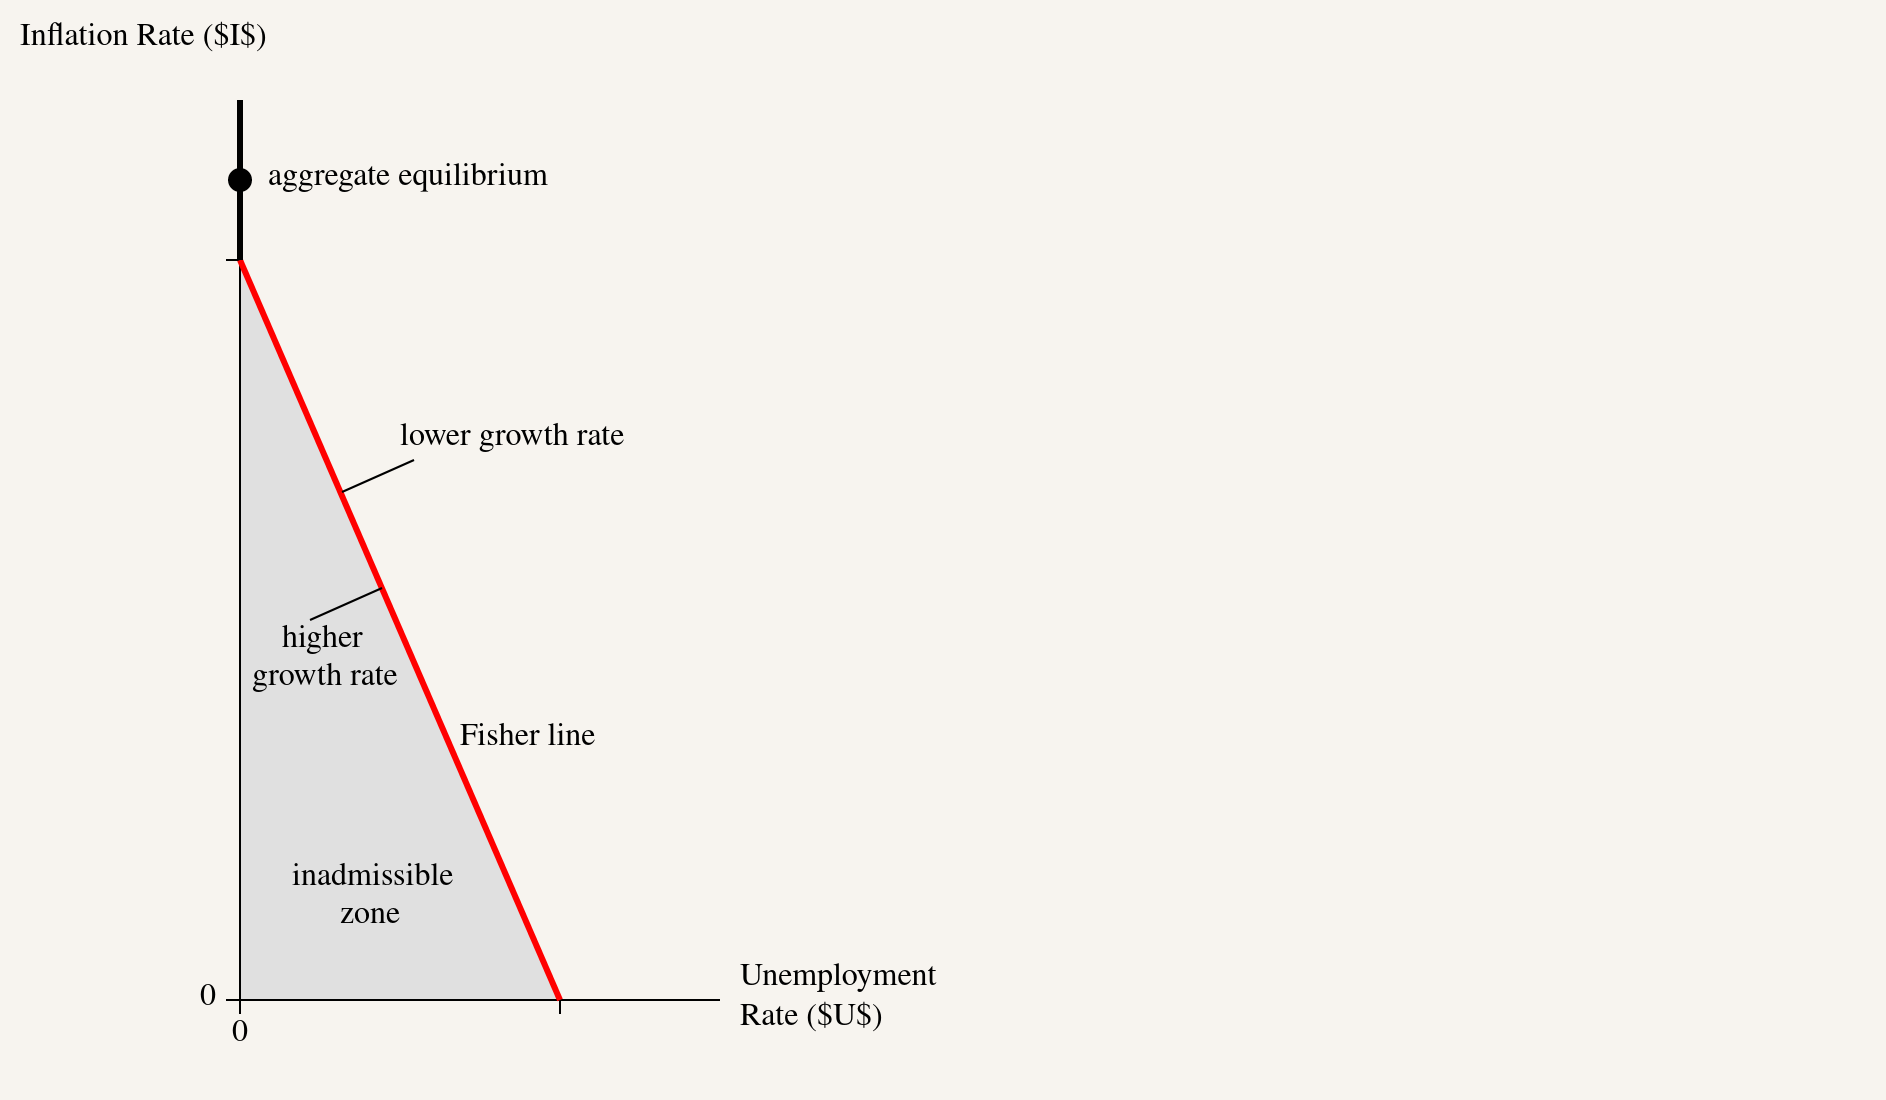
\includegraphics[scale=0.28]{/01/error_model}
\caption{Error Model}
\label{fig:error_model}
\end{figure}

The most important implication is that markets only equilibriate in aggregate along the thick black
line shown in Figure \ref{fig:error_model}, i.e. that market equilibriation an inflation rate
greater than a certain positive value. Therefore our new problem is to design a currency which is
controlled to maintain a state on the thick black line.

The critical control that a monetary authority has over a currency is

\begin{figure}
\centering

\includegraphics{example}
\caption{Unemployment and Inflation for Selected Countries}
\label{fig:ui_multi}
\end{figure}

Figure \ref{fig:ui_multi} shows a relationship between unemployment and inflation data for selected
countries that we expect to be linear when growth rates are relatively constant.

Therefore our new problem is to design a currency which is controlled to maintain a
state on the thick black line. The critical control that a monetary authority has over a currency is
through the supply of money and hence though aggregate demand and the inflation rate. In Figure
\ref{fig:error_model} the left axis, inflation, is the control variable. The growth
rate remains relatively exogenous.

To control aggregate demand we need to implement a feedback control loop with a set point above the
he rate of inflation by a sufficient buffer (see Figure \ref{fig:error_model}) to handle variations
in the system. This is best done by determining a value of from past data and then responding to
changes in $F$, the
total amount of money transacted during a period of time, which can easily be measured for a digital
currency, backed up by unemployment surveys. The money supply can be precisely determined by
indexing all payments by a index set by the monetary authority. This is done by making the payment
value equal to the product of base account value and the index. In this way, the money in all
accounts increases or decreases in exact proportion to all other accounts. This would appear to
account users much the same as one sees interest payments affect the balance of bank accounts.

The error effect is caused by a faulty control system design, and explains why contemporary
economies never achieve sustained market equilibriation or full employment. This result also

\subsection{Positive Feedback Instabilities}

\subsubsection{Time Transactions}

\subsection{Inflation Feedback}

Lending transactions cover all transactions lending contracts associated with an exchange
transactions. Introducing lending transactions to our currency, we find a run-away positive feedback
loop, where increases in inflation rates causes increases in real interest rates (Fisher effect),
that if unconstrained result in the reduction of profits of productive enterprises that results in
decreases in the growth rate and increases in the unemployment rate. This feedback can be identified
in unemployment and inflation data. This feedback instability makes it impossible to sustainably
maintain state on the black line. This feedback instability is caused by contracts nominated in
nominal dollar values, and is solved by indexing contracts with a contract index along the lines of
the Unidad de Formento in Chile. The result is that stable black line state can be maintained.

Introducing external transactions, we note that the exchange rate is exactly equal to the ratio of
inflows of currency to outflows of currency. There exists a negative feedback process (Cassel) these
inflows respond to deviations of the relative price levels in the two currencies to change the ratio
of inflows to outflows to equilibriate the exchange rate to purchasing price parity. At PPP
equilibrium, interactions between two currencies, become roughly equivalent to exchange
transactions. This stable state, however, contradicts past records of exchange rates. We deal with
this in the following paragraph.

\begin{figure}
\centering

\includegraphics{example}
\caption{Inflation Feedback}
\label{fig:inflation_feedback}
\end{figure}

\subsection{Contract Transactions}

Contract transactions are used by banks to create bank accounts. Transfers of the value in bank
accounts between different banks are accounted for by adjusting the debt relationship between those
banks using contract transactions. Bank account debts are generally not completely backed by
currency accounts. The result is a control problem, because if a large proportion money is held
outside currency accounts, it because difficult for the currencies monetary authority to control
aggregate demand.

Contractural transactions have both a stabilizing negative feedback effect through the exchange part
of the transaction, but also can have destabilizing positive feedback runaway effects through
increases in prices bring more participants into the market, thereby pushing up prices further.
Whether the negative of positive feedback plays a dominant role depends on circumstances. Also,
contract transactions are recursive and extensible and so it is possible that new kinds of
transactions that can cause unpredictable interactions with the other classes of transactions, and
therefore introduce unpredicted control problems. The danger becomes more acute if digital
currencies that are designed specifically for Ponzi-like effects and interact with other currencies
through an exchange rate are allowed to operate in the economy.

Financial bubbles occur when positive feedback becomes dominant, often resulting in sudden changes
that are hard to predict and control. This is an example where the control problem is a result of
the aggregate effects of markets (the plant) rather than the control system itself. These effects
depend on the existance of contract transactions being implicitly, in the case of paper currency and
other digital currencies, or explicitly.

\subsection{External Transactions}

\subsection{Interactions of Contract Transactions with External Transactions}

There is also considerable evidence that monetary flows across the external exchange rate boundary
are volatile, and not subject to the stabilizing exchange rate feedback process present in exchange
transactions. Contractural transactions have a sufficiently strong effect on the exchange rate such
that it does not remain in equilibrium.

\subsection{Review of Transaction Interactions}

We now have the theoretical tools to build a digital currency that controls an economy for
sustained and stable equilibriation of aggregate supply and demand. We require sufficiently large
positive inflation rates to provide sufficient redundancy for the equilibriation of aggregate supply
and demand. The results in the requirement to handle the interaction between exchange transactions
and time transactions by requiring the use of a unit of account of constant purchasing power.

In the absence of capital flows, external currencies self-regulate. Contract transactions interact
with exchange transactions by introducing the possibility of discontinuities which can disrupt the
control of aggregate equilibrium. Contract transactions also interact with external transactions by
destabilizing the self-regulation process of external transactions. Contract transactions also
disrupt the control of aggregate demand.

\subsection{Control Solutions and Resiliance}

The two requirements for a stable equilibriating economy is the use of a unit of account for all
contracts, and the prevention of capital transactions.

Calculating an accurate index for the unit of account requires a record of payments and goods
categories for each exchange transaction. All repayments are associated with a contract frame, which
determines at the time a contract is agreed upon, the money quantities to be repaid in units of
account. Also, repayments can only be made to the account from which payments are originally made.

The exchange rate is set at purchasing price parity between the two currencies, which is the ratio
of the price levels of the two currencies. The purchasing price parity should be close to the
self-regulating exchange rate under the conditions specified above.

With no contract transactions, aggregate demand can be precisely and directly controlled through an
exchange index.  The exchange index sets the purchasing value in accounts relative to an accounts
base value. The purchasing value is a product of the base value and the exchange index. An increase
in the exchange index increases the amount of all accounts in proportion. In general, the base value
of an account is hidden, and account users will see increases in their account purchasing value
closly in line with the inflation rate. The exchange index is the control variable and is generally
calculated from the sum of payments for exchange transactions over a given period.  

\begin{figure}
\centering

\includegraphics{example}
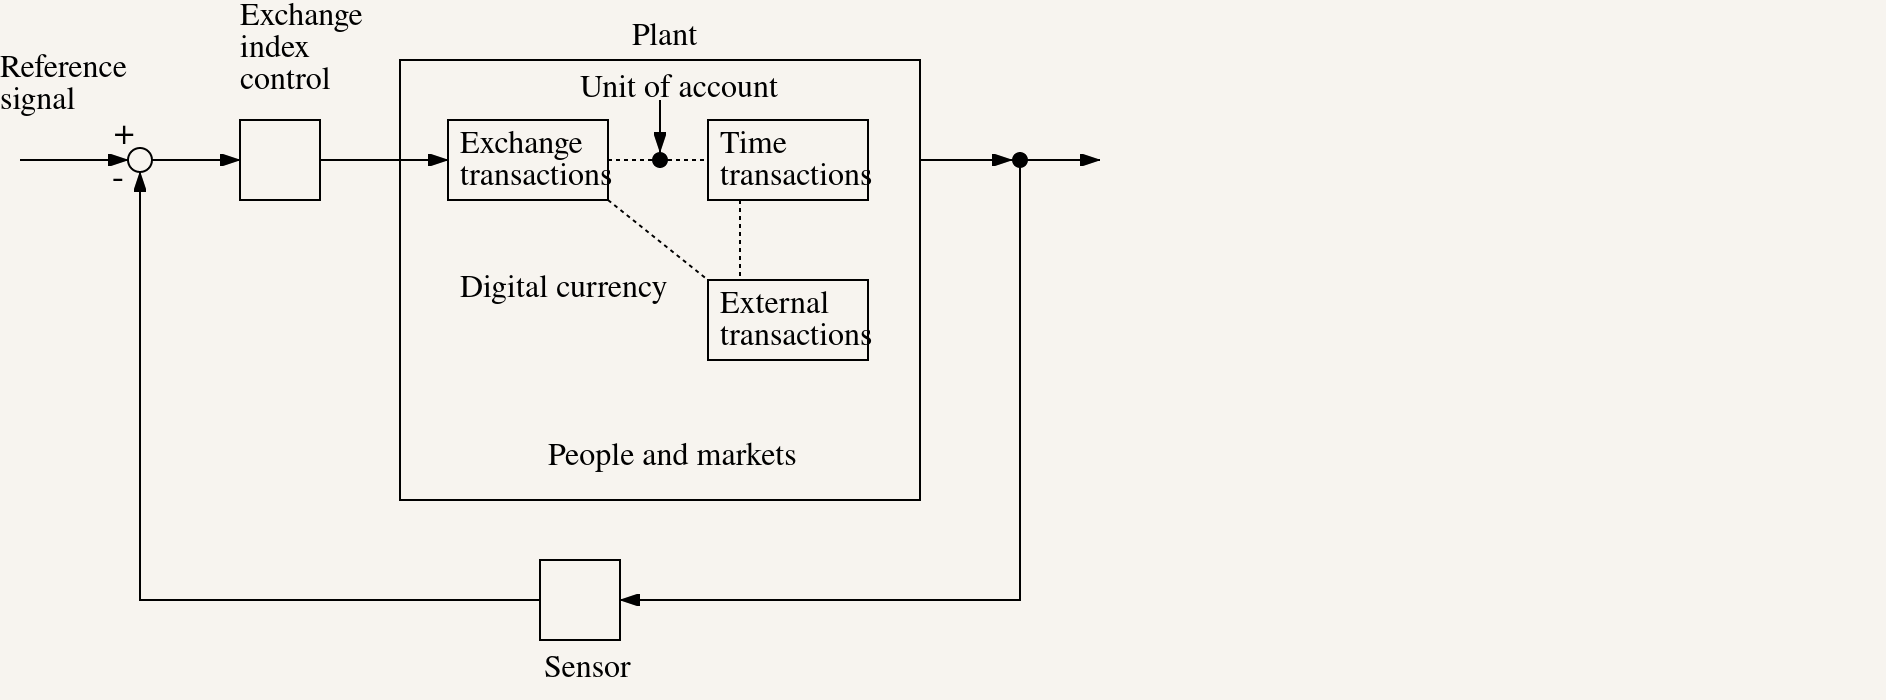
\includegraphics[scale=0.28]{/01/control_solution}
\caption{Control System Design Solution}
\label{fig:control_solution}
\end{figure}

Figure \ref{fig:control_solution} shows the control solution, with the interactions between the
classes of transactions designed to allow the aggregate price level to change without feedback
interference, with contract transactions removed to prevent financial discontinuities and to allow
the exchange rate to interact well with exchange and time transactions, and to allow direct control
of aggregate demand through an exchange index.
